\documentclass[11pt,a4paper]{article}

% Pakiety kodowania i języka polskiego
\usepackage[utf8]{inputenc}
\usepackage[T1]{fontenc}
\usepackage[polish]{babel}
\usepackage{lmodern}

% Układ strony i marginesy
\usepackage[margin=2.2cm]{geometry}
\usepackage{parskip}
\usepackage{fancyhdr}
\usepackage{lastpage}

% Grafika, tabele i kolory
\usepackage{graphicx}
\usepackage{float}
\usepackage{booktabs}
\usepackage{tabularx}
\usepackage[table,xcdraw]{xcolor}
\usepackage{caption}

% Formatowanie kodu SQL
\usepackage{listings}

% Hiperłącza
\usepackage{hyperref}
\hypersetup{
    colorlinks=true,
    linkcolor=blue!60!black,
    urlcolor=blue!60!black,
    pdftitle={Inżynieria Oprogramowania - Przesyłki kurierskie - Etap 1},
}

% Kolory niestandardowe
\definecolor{aghgreen}{RGB}{0, 105, 60}
\definecolor{aghred}{RGB}{167, 25, 48}
\definecolor{codebg}{RGB}{248, 249, 250}
\definecolor{codeframe}{RGB}{220, 224, 228}

% Konfiguracja stylu dla pliku schema.sql
\lstdefinestyle{sqlstyle}{
    language=SQL,
    backgroundcolor=\color{codebg},
    frame=single,
    rulecolor=\color{codeframe},
    basicstyle=\ttfamily\footnotesize,
    keywordstyle=\color{blue!75!black}\bfseries,
    stringstyle=\color{aghred},
    commentstyle=\color{gray}\itshape,
    numbers=left,
    numberstyle=\tiny\color{gray},
    stepnumber=1,
    numbersep=8pt,
    showstringspaces=false,
    breaklines=true,
    literate={ą}{{\k{a}}}1 {ć}{{\'c}}1 {ę}{{\k{e}}}1 {ł}{{\l{}}}1 {ń}{{\'n}}1 {ó}{{\'o}}1 {ś}{{\'s}}1 {ż}{{\.z}}1 {ź}{{\'z}}1
             {Ą}{{\k{A}}}1 {Ć}{{\'C}}1 {Ę}{{\k{E}}}1 {Ł}{{\L{}}}1 {Ń}{{\'N}}1 {Ó}{{\'O}}1 {Ś}{{\'S}}1 {Ż}{{\.Z}}1 {Ź}{{\'Z}}1
}

% Nagłówek i stopka
\pagestyle{fancy}
\fancyhf{}
\lhead{\footnotesize \textbf{Inżynieria Oprogramowania} -- Przesyłki kurierskie}
\rhead{\footnotesize AGH WEAIiIB -- Informatyka i Systemy Inteligentne (2026/2027)}
\cfoot{\footnotesize Strona \thepage\ z \pageref{LastPage}}
\renewcommand{\headrulewidth}{0.4pt}
\renewcommand{\footrulewidth}{0.4pt}

\begin{document}

% -------------------------------------------------------------------
% STRONA TYTUŁOWA / NAGŁÓWEK DOKUMENTU
% -------------------------------------------------------------------
\begin{center}
    {\Large \textbf{Akademia Górniczo-Hutnicza im. Stanisława Staszica w Krakowie}}\\[0.2cm]
    {\normalsize Wydział Elektrotechniki, Automatyki, Informatyki i Inżynierii Biomedycznej}\\
    {\normalsize Kierunek: Informatyka i Systemy Inteligentne}\\[0.8cm]
    
    \rule{\textwidth}{1.2pt}\\[0.4cm]
    {\LARGE \textbf{System obsługi przesyłek kurierskich i dostaw}}\\[0.2cm]
    {\large Etap 2 (21.X): Architektura systemu, przypadki użycia oraz struktury danych}\\[0.2cm]
    \rule{\textwidth}{1.2pt}\\[0.6cm]
\end{center}

\begin{table}[H]
\centering
\renewcommand{\arraystretch}{1.25}
\begin{tabularx}{\textwidth}{>{\bfseries}l X}
    Przedmiot: & Inżynieria Oprogramowania (Semestr zimowy 2026/2027) \\
    Prowadzący: & dr inż. Marek Zachara \\
    Temat projektu: & Temat nr 3 -- Przesyłki kurierskie \\
    Skład zespołu: & Marcel Kosmala, Igor Krzystek, Filip Kontek \\
    Data prezentacji: & 21 października 2026 r. \\
\end{tabularx}
\end{table}

\vspace{0.3cm}
\tableofcontents
\newpage

% -------------------------------------------------------------------
% SEKCJA 1: OPIS SYSTEMU I ZAŁOŻENIA
% -------------------------------------------------------------------
\section{Wprowadzenie i główny zakres funkcjonalny}

Celem projektu jest zaprojektowanie systemu informatycznego wspierającego proces zamawiania oraz dostarczania przesyłek i posiłków. System integruje pracę trzech głównych ról użytkowników, zapewniając dedykowane procesy biznesowe (workflow) oraz kontrolę uprawnień:

\begin{itemize}
    \item \textbf{Klient (\texttt{CLIENT})} -- przegląda ofertę dostawców (z możliwością wyszukiwania lokali w pobliżu), kompletuje koszyk, składa i opłaca zamówienia, śledzi status realizacji w czasie rzeczywistym, a po dostarczeniu wystawia ocenę (1--5) wraz z komentarzem dla dostawcy oraz kuriera.
    \item \textbf{Dostawca (\texttt{VENDOR})} -- zarządza katalogiem swoich produktów (dodawanie, edycja, ukrywanie pozycji w ofercie), odbiera nowe zamówienia, decyduje o ich akceptacji bądź odrzuceniu oraz aktualizuje stan przygotowania paczki.
    \item \textbf{Kurier (\texttt{COURIER})} -- zarządza swoim statusem dostępności, cyklicznie raportuje swoją bieżącą lokalizację GPS, przegląda przydzielone zlecenia, odbiera przygotowane zamówienia z lokalu dostawcy i potwierdza ich dostarczenie do klienta.
\end{itemize}

\subsection{Cykl życia zamówienia (Automat stanów)}
Każde zamówienie w systemie jest zarządzane przez deterministyczny automat stanów zapisywany w bazie danych:
\begin{center}
    \texttt{ORDERED} $\rightarrow$ \texttt{ACCEPTED} $\rightarrow$ \texttt{PREPARATION} $\rightarrow$ \texttt{SHIPPING} $\rightarrow$ \texttt{DELIVERED}
\end{center}
Dodatkowo automat obsługuje stany wyjątkowe:
\begin{itemize}
    \item \texttt{CANCELLED} -- anulowanie zamówienia przez klienta (możliwe wyłącznie w stanie początkowym \texttt{ORDERED}, zanim dostawca rozpocznie realizację),
    \item \texttt{REJECTED} -- odrzucenie zamówienia przez dostawcę przed jego przyjęciem do realizacji.
\end{itemize}

% -------------------------------------------------------------------
% SEKCJA 2: ARCHITEKTURA SYSTEMU
% -------------------------------------------------------------------
\section{Architektura systemu}

System został zaprojektowany w oparciu o modularną architekturę trójwarstwową z wyraźnym podziałem na warstwę prezentacji (\textbf{Frontend}), warstwę logiki biznesowej (\textbf{Backend}), warstwę składowania danych (\textbf{PostgreSQL + PostGIS}) oraz integracje zewnętrzne. Ogólny schemat architektury przedstawia Rysunek~\ref{fig:architektura}.

\begin{figure}[H]
    \centering
    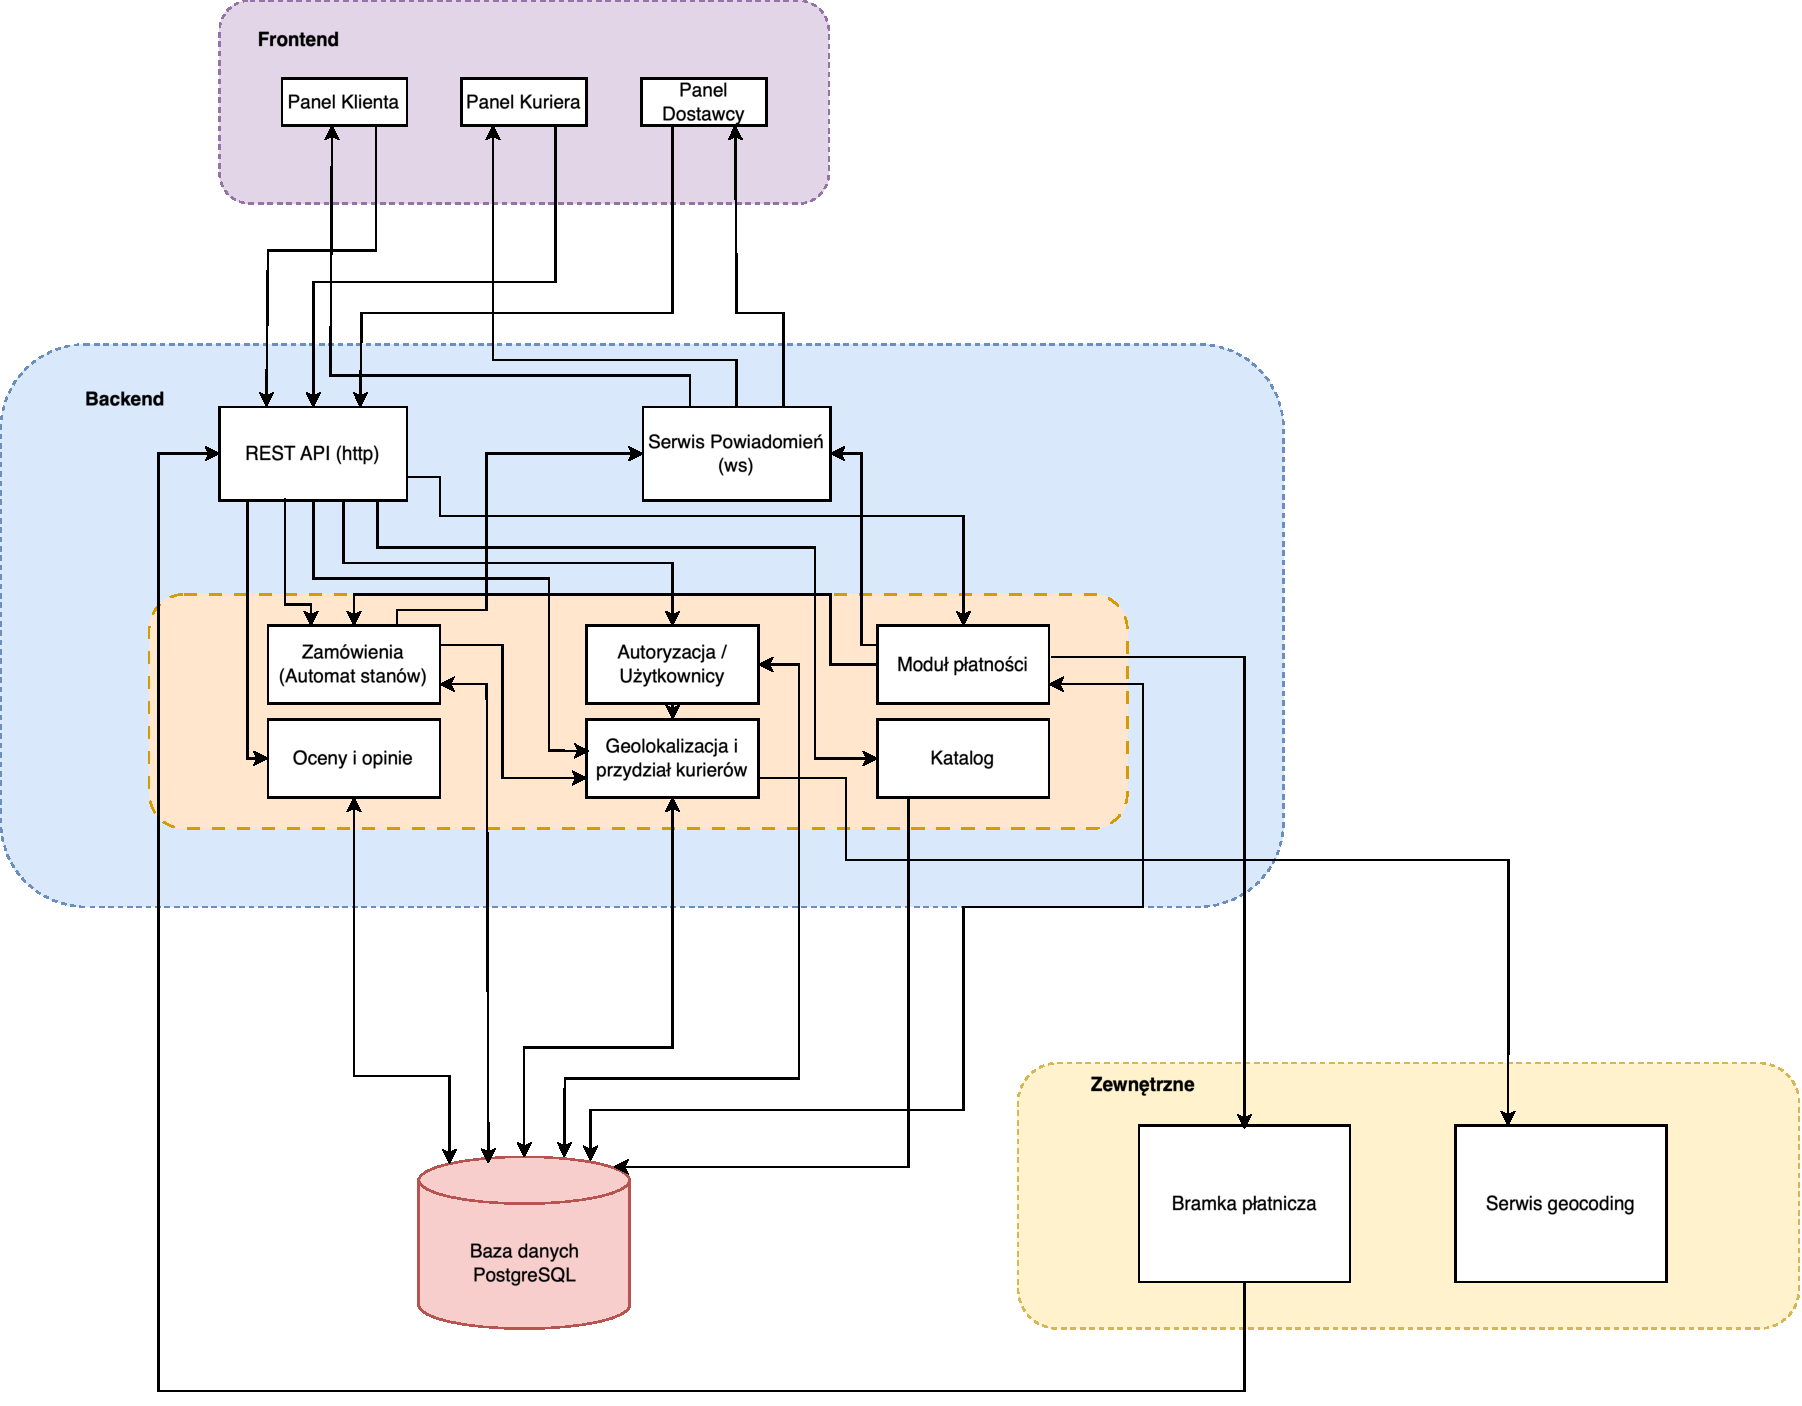
\includegraphics[width=0.92\textwidth]{architecture_diagram.pdf}
    \caption{Logiczna architektura systemu przesyłek kurierskich wraz z przepływem danych między modułami.}
    \label{fig:architektura}
\end{figure}

\subsection{Opis głównych komponentów i przepływów}
\begin{enumerate}
    \item \textbf{Warstwa Frontend:} Podzielona na trzy dedykowane widoki: \textit{Panel Klienta}, \textit{Panel Dostawcy} oraz \textit{Panel Kuriera}. Komunikuje się z serwerem synchronicznie poprzez protokół HTTP (\texttt{REST API}) oraz asynchronicznie za pomocą połączenia dwukierunkowego WebSocket (\texttt{Serwis Powiadomień (ws)}), co pozwala na natychmiastowe dostarczanie powiadomień o zmianach statusu zamówienia do każdej ze stron.
    \item \textbf{Moduły domenowe Backendu:}
    \begin{itemize}
        \item \textbf{Zamówienia (Automat stanów)} -- centralny moduł koordynujący przejścia między stanami zamówienia, wyzwalający przydział kuriera oraz wysyłkę powiadomień.
        \item \textbf{Geolokalizacja i przydział kurierów} -- odpowiada za zamianę adresów tekstowych na współrzędne geograficzne we współpracy z zewnętrznym \textit{Serwisem geocoding} (np. API Nominatim / OpenStreetMap) oraz za wyszukiwanie najbliższego dostępnego kuriera względem lokalizacji dostawcy za pomocą zapytań przestrzennych PostGIS.
        \item \textbf{Katalog} -- obsługuje operacje CRUD na ofercie produktów poszczególnych dostawców.
        \item \textbf{Moduł płatności} -- integruje system z zewnętrzną \textit{Bramką płatniczą} i odbiera zwrotne potwierdzenia transakcji (webhooki), aktualizując status płatności i powiadamiając o tym odpowiednie strony.
        \item \textbf{Autoryzacja / Użytkownicy} -- zarządza rejestracją, logowaniem, sesjami użytkowników oraz profilami ról.
        \item \textbf{Oceny i opinie} -- weryfikuje uprawnienia do wystawienia oceny (tylko dla zamówień ze statusem \texttt{DELIVERED}, maksymalnie jedna ocena dla kuriera i jedna dla dostawcy na zamówienie) oraz aktualizuje średnie oceny profilowe.
    \end{itemize}
\end{enumerate}

\newpage
% -------------------------------------------------------------------
% SEKCJA 3: PRZYPADKI UŻYCIA (UML USE-CASE)
% -------------------------------------------------------------------
\section{Analiza przypadków użycia (UML Use-Cases)}

Model funkcjonalny systemu został podzielony na diagram przeglądowy (Rysunek~\ref{fig:uc_ogolny}), który definiuje hierarchię aktorów i główne procesy, oraz trzy szczegółowe diagramy prezentujące perspektywę każdej roli.

\begin{figure}[H]
    \centering
    \includegraphics[width=0.88\textwidth]{UC1_ogolny.pdf}
    \caption{Ogólny diagram przypadków użycia systemu przesyłek kurierskich.}
    \label{fig:uc_ogolny}
\end{figure}

Na diagramie ogólnym (Rysunek~\ref{fig:uc_ogolny}) wyodrębniono niezalogowanego aktora \textit{Gość} (uprawnionego do rejestracji konta) oraz abstrakcyjnego aktora \textit{Użytkownik}, po którym dziedziczą role \textit{Klient}, \textit{Dostawca} i \textit{Kurier}. Wszystkie te role współdzielą przypadki użycia \textit{Zaloguj się} oraz \textit{Przeglądaj powiadomienia}.

\subsection{Perspektywa Klienta}
Szczegółowe przypadki użycia dla roli Klienta prezentuje Rysunek~\ref{fig:uc_klient}. Podczas przeglądania oferty klient może opcjonalnie (\texttt{<<extend>>}) filtrować dostawców w pobliżu oraz dodawać produkty do koszyka. Złożenie zamówienia bezwarunkowo (\texttt{<<include>>}) wymaga podania adresu dostawy (walidowanego przez zewnętrzny \textit{Serwis geocoding}), opłacenia zamówienia poprzez \textit{Bramkę płatniczą} oraz wysłania powiadomienia do dostawcy.

\begin{figure}[H]
    \centering
    \includegraphics[width=0.98\textwidth]{UC2_klient.pdf}
    \caption{Diagram przypadków użycia -- perspektywa Klienta.}
    \label{fig:uc_klient}
\end{figure}

\subsection{Perspektywa Dostawcy i Kuriera}
Rysunek~\ref{fig:uc_dostawca} oraz Rysunek~\ref{fig:uc_kurier} przedstawiają procesy realizowane przez Dostawcę oraz Kuriera:
\begin{itemize}
    \item \textbf{Akceptacja i przydział kuriera:} Zaakceptowanie zamówienia przez dostawcę automatycznie uruchamia przypadek \textit{Przydziel najbliższego dostępnego kuriera} (relacja \texttt{<<include>>}), który wybiera dostępnego kuriera znajdującego się najbliżej lokalu dostawcy i wysyła powiadomienia o zmianie statusu zarówno do Klienta, jak i do Kuriera.
    \item \textbf{Realizacja dostawy i telemetria:} Kurier w trakcie dostępności cyklicznie przesyła swoją pozycję GPS (\textit{Aktualizuj lokalizację}), a przy odbiorze paczki od dostawcy (\texttt{SHIPPING}) oraz potwierdzeniu doręczenia (\texttt{DELIVERED}) system automatycznie rozsyła powiadomienia do pozostałych uczestników procesu.
\end{itemize}

\begin{figure}[H]
    \centering
    \includegraphics[width=0.92\textwidth]{UC3_dostawca.pdf}
    \caption{Diagram przypadków użycia -- perspektywa Dostawcy.}
    \label{fig:uc_dostawca}
\end{figure}

\begin{figure}[H]
    \centering
    \includegraphics[width=0.92\textwidth]{UC4_kurier.pdf}
    \caption{Diagram przypadków użycia -- perspektywa Kuriera.}
    \label{fig:uc_kurier}
\end{figure}

\newpage
% -------------------------------------------------------------------
% SEKCJA 4: STRUKTURA DANYCH I BAZA RELACYJNA
% -------------------------------------------------------------------
\section{Projekt struktury danych (Baza relacyjna PostgreSQL + PostGIS)}

Dane persystentne składowane są w relacyjnej bazie danych PostgreSQL wzbogaconej o rozszerzenie przestrzenne \textbf{PostGIS}. Relacje pomiędzy tabelami oraz krotności powiązań kluczy obcych przedstawia diagram ERD na Rysunku~\ref{fig:erd}.

\begin{figure}[H]
    \centering
    % page=2 wyświetla wersję diagramu z opisanymi nazwami kluczy obcych i krotnościami (1, 0..*, 0..1)
    \includegraphics[page=2,width=1.0\textwidth]{database_diagram.pdf}
    \caption{Diagram związków encji (ERD) z krotnościami relacji i kluczami obcymi.}
    \label{fig:erd}
\end{figure}

\subsection{Kluczowe decyzje projektowe w strukturze bazy danych}
\begin{itemize}
    \item \textbf{Obsługa danych geograficznych (\texttt{PostGIS}):} Lokalizacja lokalu dostawcy (\texttt{vendor\_profiles.location}), bieżąca pozycja kuriera (\texttt{courier\_profiles.current\_location}) oraz punkt docelowy zamówienia (\texttt{orders.delivery\_location}) używają typu \texttt{geography(Point, 4326)} (układ współrzędnych WGS 84). Na kolumnie \texttt{current\_location} założono indeks przestrzenny \texttt{GIST} (\texttt{idx\_courier\_location}), co gwarantuje błyskawiczne wyszukiwanie najbliższego kuriera.
    \item \textbf{Integralność cenowa zamówień:} Tabela \texttt{order\_items} przechowuje kolumnę \texttt{unit\_price}, która zamraża cenę produktu w momencie zakupu -- późniejsza edycja ceny przez dostawcę w tabeli \texttt{products} nie zmienia historycznych kwot zamówień.
    \item \textbf{Więzy spójności ocen (\texttt{ratings}):} Zastosowano ograniczenie unikalności \texttt{UNIQUE (order\_id, target\_role)}, dzięki czemu klient w ramach jednego zamówienia może wystawić dokładnie jedną ocenę dostawcy (\texttt{VENDOR}) oraz jedną ocenę kurierowi (\texttt{COURIER}).
    \item \textbf{Trwałość powiadomień (\texttt{notifications}):} Oprócz wysyłki w czasie rzeczywistym przez WebSocket, powiadomienia są zapisywane w bazie wraz z flagą \texttt{is\_read}, co pozwala użytkownikom na odczytanie historii komunikatów po ponownym zalogowaniu.
\end{itemize}

\subsection{Skrypt definicji schematu bazy danych (DDL)}
Poniższy listing prezentuje kompletny kod SQL definiujący tabele, klucze główne i obce, ograniczenia \texttt{CHECK} oraz indeksy przestrzenne:

\lstinputlisting[style=sqlstyle]{database_schema.sql}

% -------------------------------------------------------------------
% SEKCJA 5: OPTYMALIZACJA WYDAJNOŚCI I REDIS
% -------------------------------------------------------------------
\newpage
\section{Optymalizacja lokalizacji kurierów i przydziału (Integracja z Redis)}

W trakcie prac projektowych nad modułem \textbf{Geolokalizacji i przydziału kurierów} zdiagnozowano potencjalne wąskie gardła związane z wydajnością, gdy system zostanie uruchomiony dla dużej floty kurierów w obrębie całego miasta. Problem dotyczy częstotliwości aktualizacji lokalizacji na żywo.

\subsection{Identyfikacja wąskiego gardła architektonicznego}

Pierwotne założenie, odwzorowane w tabeli \texttt{courier\_profiles}, zakładało, że aplikacja mobilna kuriera co 10 sekund wysyła do serwera swoją aktualną pozycję (GPS), co skutkowało operacją aktualizacji w głównej bazie relacyjnej: \texttt{UPDATE courier\_profiles SET current\_location = <gps>, last\_ping\_at = NOW()}. 

Takie rozwiązanie w środowisku produkcyjnym niesie za sobą poważne konsekwencje (Rysunek~\ref{fig:seq_problem}):
\begin{itemize}
    \item \textbf{Obciążenie wejścia/wyjścia (I/O) i pęcznienie bazy (Table Bloat):} Silnik PostgreSQL wykorzystuje mechanizm MVCC (Multi-Version Concurrency Control). Każda operacja \texttt{UPDATE} nie nadpisuje starych danych bezpośrednio na dysku, lecz oznacza stary wiersz jako martwy i tworzy nowy. Dla 200 kurierów wysyłających lokalizację co 10 sekund, generujemy 1200 zapytań \texttt{UPDATE} na minutę do jednej tabeli. Spowalnia to zapytania analityczne i inne procesy logiki biznesowej.
    \item \textbf{Konflikty dostępu (Race Conditions):} Jeśli w tym samym momencie do systemu spłyną dwa zamówienia dla lokali w bliskiej odległości, dwa współbieżne zapytania \texttt{SELECT} wybiorą tego samego kuriera (ponieważ posiada on wciąż status \texttt{is\_available = true}).
\end{itemize}

\begin{figure}[H]
    \centering
    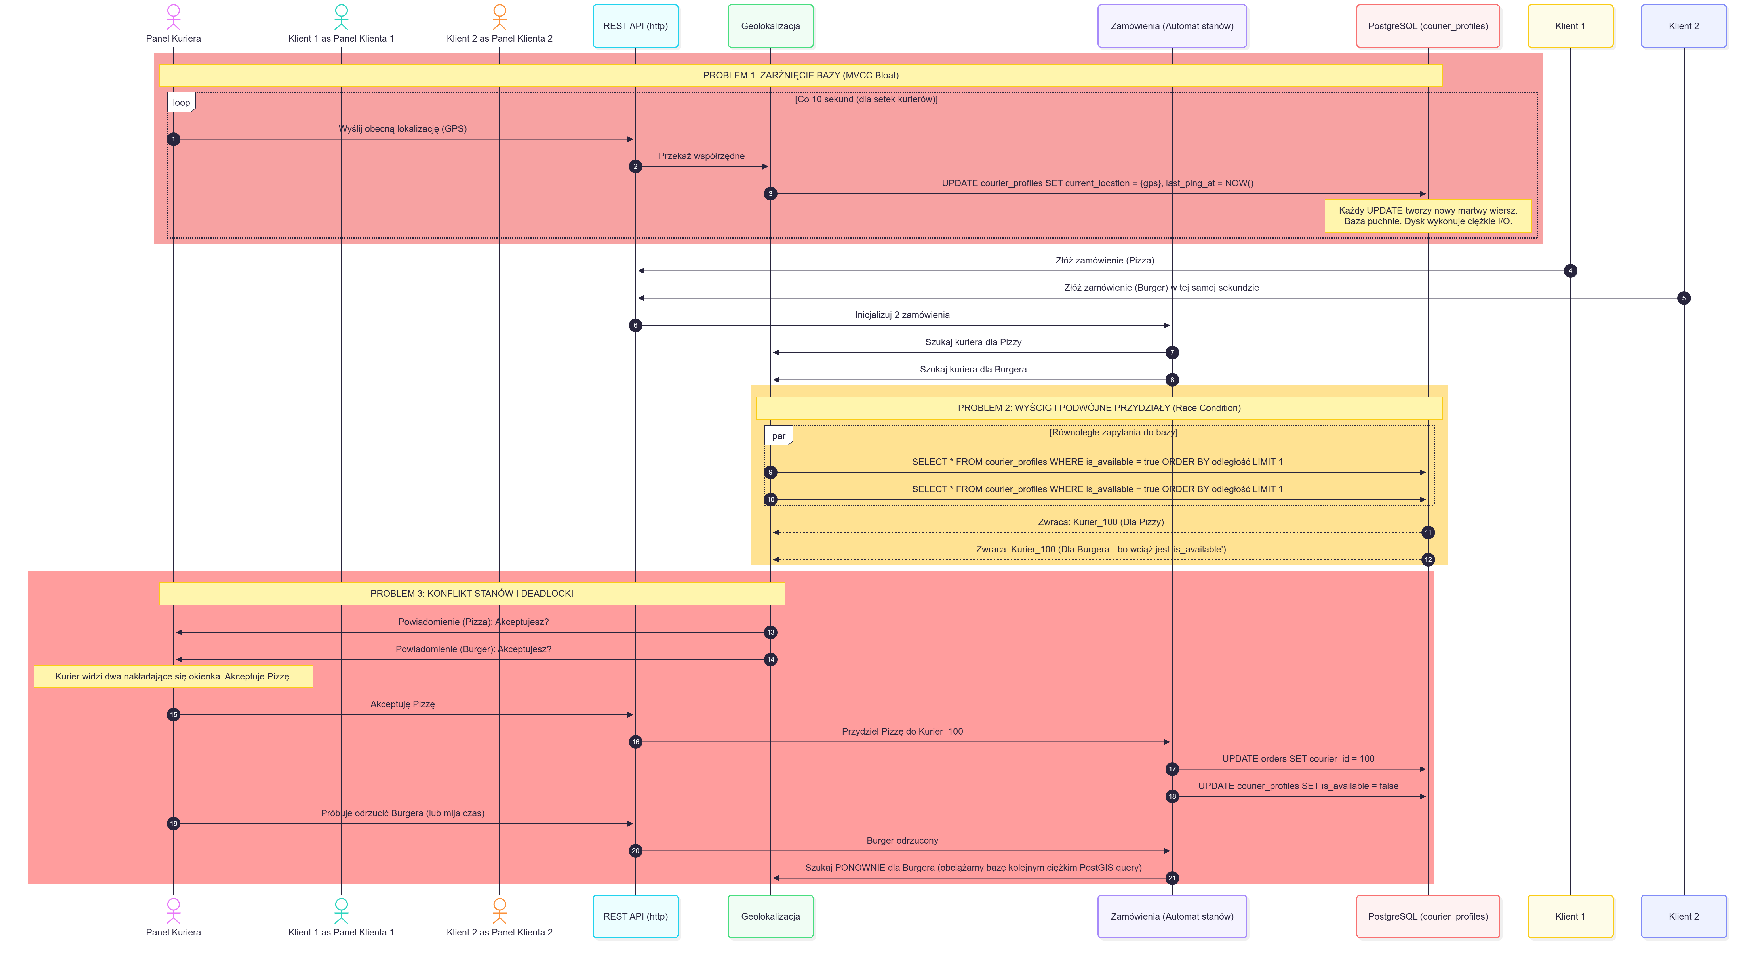
\includegraphics[width=0.95\textwidth]{couriers_problem.pdf}
    \caption{Diagram sekwencyjny uwydatniający problemy z wydajnością i współbieżnością w naiwnym podejściu do przydziału kuriera (tylko PostgreSQL).}
    \label{fig:seq_problem}
\end{figure}

\subsection{Wprowadzenie struktury in-memory (Redis)}

W celu odciążenia głównej bazy danych zaimplementowano hybrydowe rozwiązanie oparte na in-memory datastore -- \textbf{Redis}. Wykorzystano w nim specjalistyczne moduły do operacji przestrzennych. Zaktualizowaną architekturę systemu przedstawia Rysunek~\ref{fig:arch_redis}.

\begin{figure}[H]
    \centering
    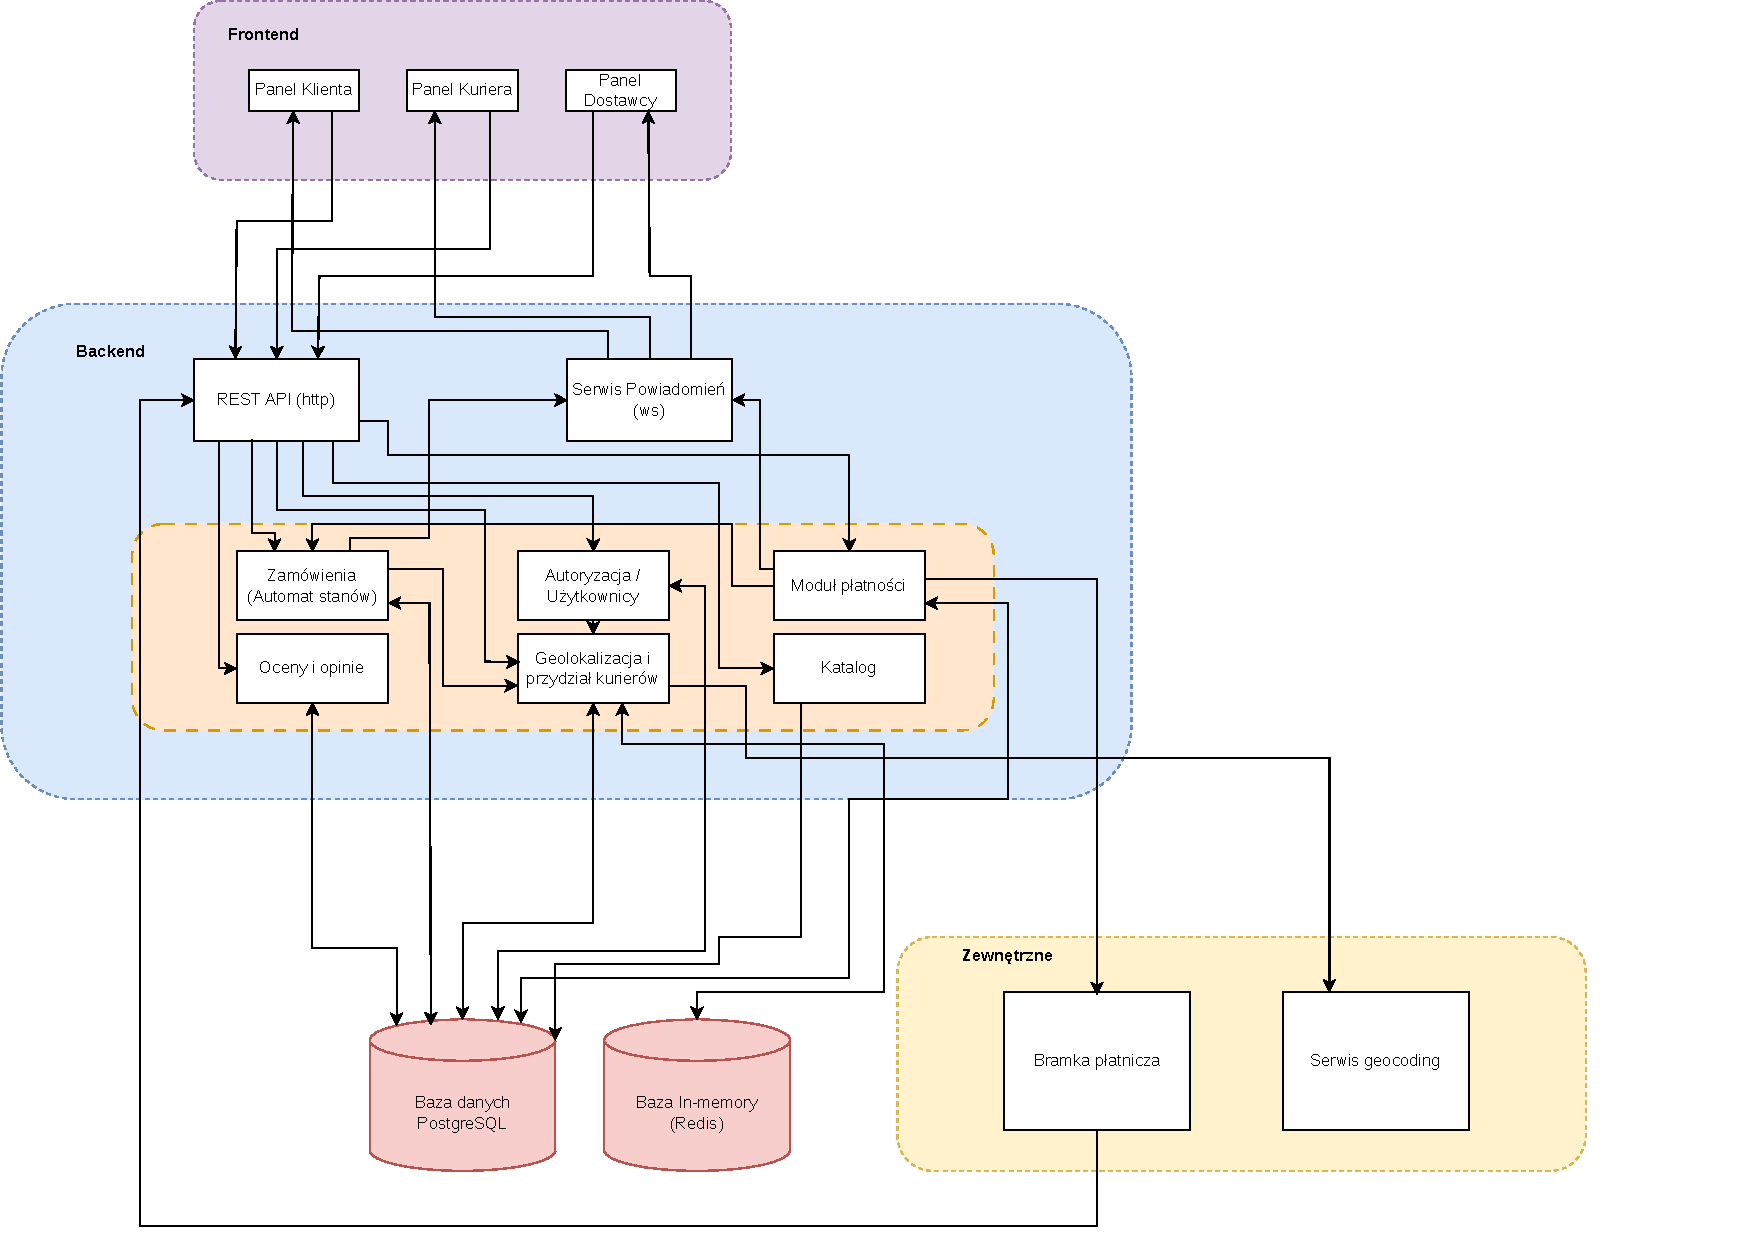
\includegraphics[width=0.92\textwidth]{architecture_with_redis.pdf}
    \caption{Zaktualizowana logiczna architektura systemu uwzględniająca bazę danych Redis dla operacji na żywo.}
    \label{fig:arch_redis}
\end{figure}

Działanie nowego, zoptymalizowanego mechanizmu:
\begin{enumerate}
    \item \textbf{Rejestrowanie pozycji (Geohash):} Pingi geolokalizacyjne od kurierów nie uderzają już bezpośrednio w PostgreSQL. Są one asynchronicznie zapisywane w Redisie za pomocą komendy \texttt{GEOADD}, która w locie przelicza koordynaty trygonometryczne na algorytm Geohash i zachowuje je w zbiorach posortowanych w pamięci RAM.
    \item \textbf{Ghost Couriers i Time-to-Live (TTL):} Aby uniknąć przydzielania zamówień kurierom, którzy zgubili zasięg, dodano równoległy zapis unikalnego klucza (np. \texttt{SET courier:100:active "1" EX 15}) z ustawionym 15-sekundowym czasem wygaśnięcia.
    \item \textbf{Soft Locking (Blokady współbieżne):} Podczas przydzielania kuriera za pomocą \texttt{GEOSEARCH}, system wykorzystuje krótki skrypt (np. w języku Lua), który atomowo sprawdza dostępność kuriera i tymczasowo go blokuje (soft lock). Gwarantuje to uniknięcie zjawiska podwójnego przydziału.
    \item \textbf{Ostateczne utrwalenie stanu:} Dopiero gdy kurier zaakceptuje zamówienie za pomocą aplikacji, system informuje o tym Automat Stanów, dokonując \textit{twardego} zapisu do relacyjnej bazy PostgreSQL (aktualizacja kolumny \texttt{courier\_id} w zamówieniu).
\end{enumerate}

Zoptymalizowany przepływ danych, wolny od rywalizacji o zasoby bazodanowe i wąskich gardeł transakcyjnych, ukazuje Rysunek~\ref{fig:seq_rozwiazanie}.

\begin{figure}[H]
    \centering
    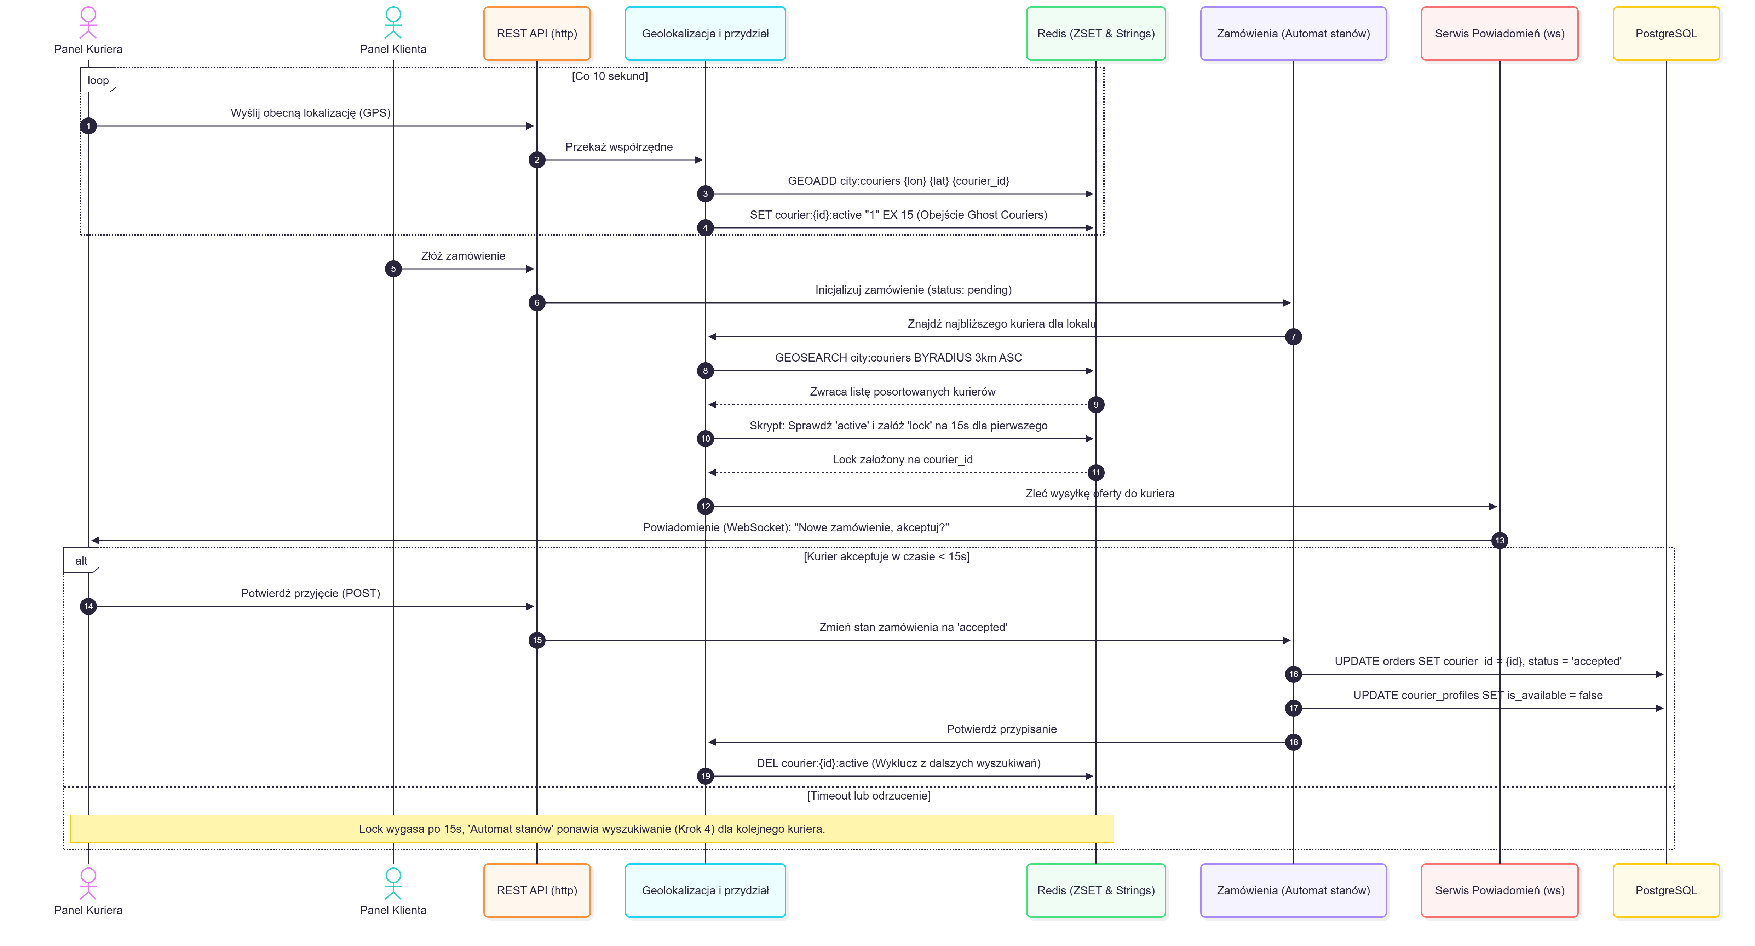
\includegraphics[width=0.95\textwidth]{couriers_solution.pdf}
    \caption{Zoptymalizowany przepływ przydziału kuriera przy wykorzystaniu zapytań geoprzestrzennych oraz soft-locków w bazie Redis.}
    \label{fig:seq_rozwiazanie}
\end{figure}



\end{document}